\documentclass[11pt]{scrartcl}

\usepackage[top=1.5cm]{geometry}
\usepackage{url}
\usepackage{float}
\usepackage{listings}
\usepackage{xcolor}
\usepackage{graphicx}

\setlength{\parindent}{0em}
\setlength{\parskip}{0.5em}

\newcommand{\youranswerhere}{[Your answer goes here \ldots]}
\renewcommand{\thesubsection}{\arabic{subsection}}

\lstdefinestyle{dmrsql}{
  language=SQL,
  basicstyle=\small\ttfamily,
  keywordstyle=\color{magenta!75!black},
  stringstyle=\color{green!50!black},
  showspaces=false,
  showstringspaces=false,
  commentstyle=\color{gray}}

\lstdefinestyle{dmrJava}{
  language=JAVA,
  basicstyle=\small\ttfamily,
  keywordstyle=\color{magenta!75!black},
  stringstyle=\color{green!50!black},
  showspaces=false,
  showstringspaces=false,
  commentstyle=\color{gray}}

\title{
  \textbf{\large Projektaufgabe 2 } \\
  Phase 2 – Legen der Basis (2.5 P) \\
  {\large Datenmanagement jenseits von Relationen}
}

\author{
 Gruppen Nummer (A8) \\
  \large Acikyol Aleyna, 12032843 \\
  \large Özcan Ahmet, 12311287 \\
  \large Sadykova Nargiz, 12129337 \\
}

\begin{document}

\maketitle\thispagestyle{empty}

Dieses Reporting Template dient der Vorbereitung der Abgabe von Phase 2.

\subsection*{Alternativer Import für Ansatz 2 (0.5 Punkte)}

Zeigen Sie das create table Statement für $A$ oder $B$. 

\begin{lstlisting}[style=dmrsql]
CREATE TABLE A_ROW (
    i INT NOT NULL,
    row DOUBLE PRECISION[] NOT NULL
);
\end{lstlisting}

Zeigen Sie, wie die Matrizen $A$ und $B$ des Toy Examples für Ansatz 2 in der DB aussehen.

\youranswerhere{}

\subsection*{Ansatz 2 (0.5 Punkte):}

Geben Sie den Code der Funktion \texttt{dotproduct()} bzw. Ihrer Lösung für Ansatz 2 an.

\begin{lstlisting}[style=dmrsql]
[dotproduct() UDF ...]
\end{lstlisting}

Zeigen Sie für das Toy Example, dass $C$ korrekt berechnet wird (z.B. via Screenshot).

\youranswerhere{}

\subsection*{Benchmark Definition (0.5 P):}

Als Metrik verwenden wir die \textbf{Zeit für eine Matrixmultiplikation} (Durchschnitt über 3 Wiederholungen).
Die drei Ansätze werden für alle Kombinationen $(L, S)$ verglichen.
Die Matrizen haben die Dimensionen $A \in \mathbb{R}^{(l-1) \times l}$ und $B \in \mathbb{R}^{l \times (l-1)}$.

\begin{table}[h]
	\centering
	\begin{tabular}{ c c c }
		\hline
		Parameter & Werte & Kommentar \\
		\hline
		L & $\{8,\, 16,\, 32,\, 64,\, 128,\, 256\}$ & Zweierpotenzen ab $2^3$; passt vollständig in den Hauptspeicher \\
		S & $\{0.1,\, 0.3,\, 0.5,\, 0.7,\, 0.9\}$ & Sparsity-Werte; Matrix im Allgemeinen eher dicht besetzt \\
		\hline
	\end{tabular}
	\caption{Getestete Matrixgrößen L und Sparsity-Werte S (30 Kombinationen)}
	\label{tab:MatrixgrößenLUndSparsityWerteS}
\end{table}

\subsubsection*{Auswertung (0.5 P)}

Stellen Sie Ihre Messergebnisse grafisch dar.

\begin{figure}[H]
	\centering
	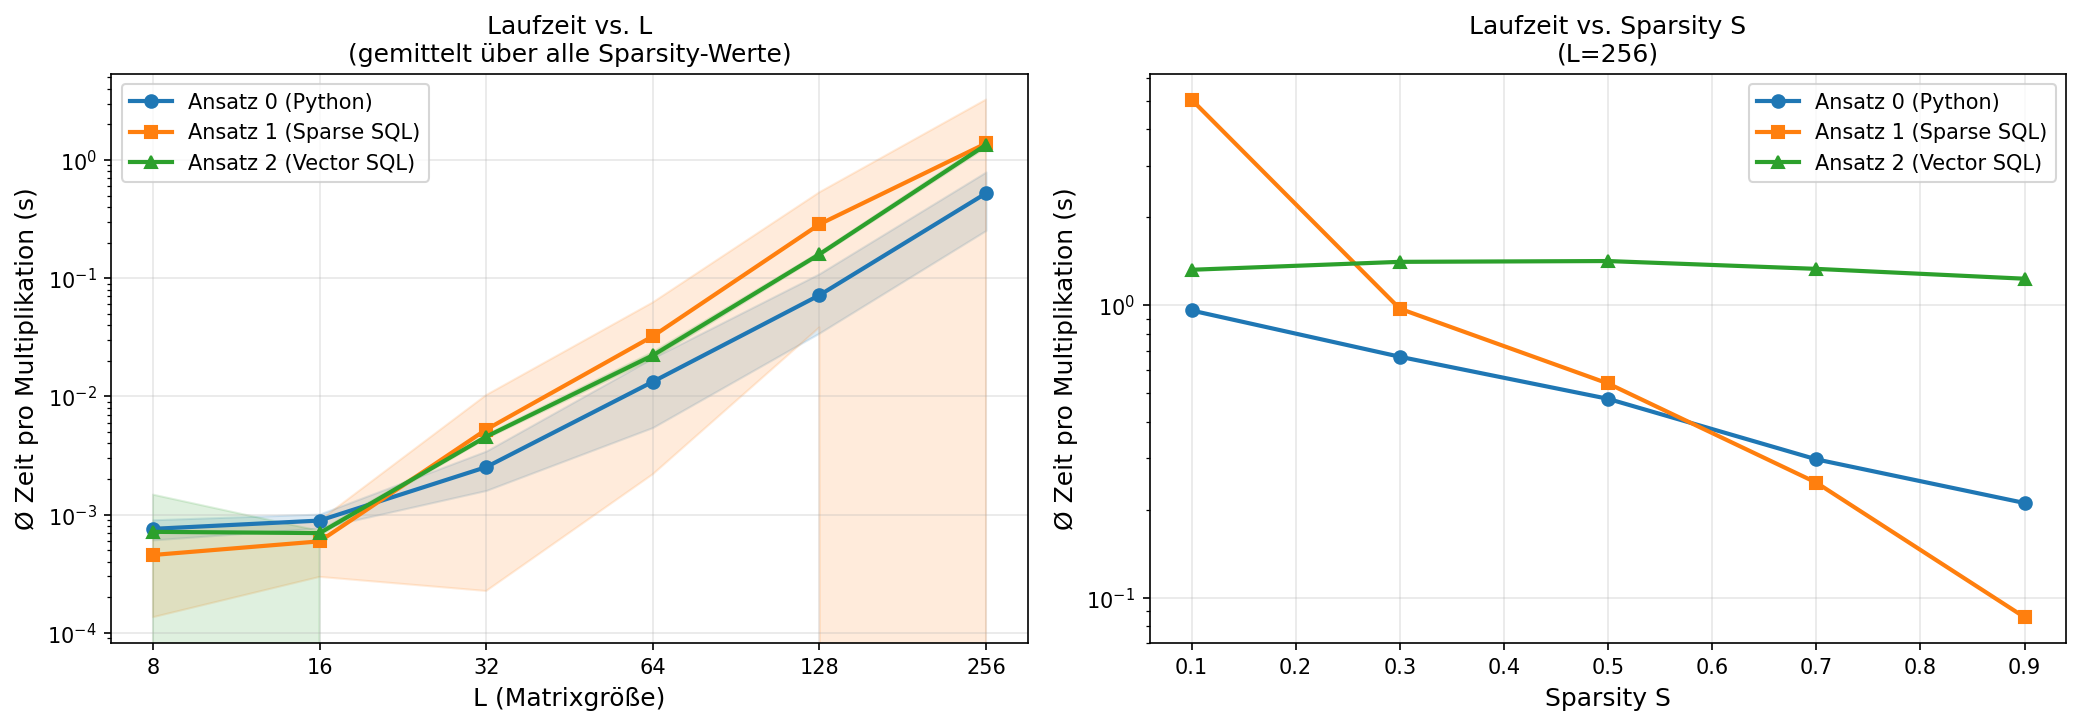
\includegraphics[width=\textwidth]{results}
	\caption{Laufzeit der drei Ansätze: links gemittelt über alle Sparsity-Werte in Abhängigkeit von $L$; rechts in Abhängigkeit von $S$ bei $L=256$.}
	\label{fig:results}
\end{figure}

\textbf{Fazit:}
Die Messungen zeigen deutliche Unterschiede im Verhalten der drei Ansätze:

\begin{itemize}
  \item \textbf{Ansatz 1 (Sparse SQL)} profitiert stark von hoher Sparsity: Bei $L=256$ und $S=0.1$ (dichte Matrix) benötigt er ca.\ 5\,s, bei $S=0.9$ (dünne Matrix) nur ca.\ 0.09\,s.
        Bei dichter Besetzung ist der Join über die Nicht-Null-Einträge sehr teuer.
  \item \textbf{Ansatz 2 (Vector SQL)} ist weitgehend \textbf{sparsity-unabhängig}, da \texttt{dotproduct()} stets alle $l$ Array-Elemente durchläuft.
        Die Laufzeit bei $L=256$ beträgt konstant ca.\ 1.3\,s, unabhängig von $S$.
        Bei dichter Matrix ist Ansatz 2 daher besser als Ansatz 1; bei sehr dünner Matrix ist Ansatz 1 deutlich schneller.
  \item \textbf{Ansatz 0 (Python)} überträgt die Daten aus der DB und berechnet das Ergebnis clientseitig.
        Er überspringt Nulleinträge und skaliert daher ähnlich wie Ansatz 1 mit der Sparsity.
        Bei $L=256$ liegt er zwischen beiden DB-Ansätzen und ist bei mittlerer Sparsity konkurrenzfähig.
\end{itemize}

Insgesamt eignet sich \textbf{Ansatz 1} am besten für dünn besetzte Matrizen, während \textbf{Ansatz 2} bei dichten Matrizen vorzuziehen ist.
\textbf{Ansatz 0} zeigt, dass clientseitige Python-Berechnung bei kleinen bis mittleren Matrixgrößen durchaus mit datenbankinternen Ansätzen mithalten kann.


\subsection*{Zeitmamagement}

Benötigte Zeit pro Person (nur Phase 1): \textbf{Acikyol Aleyna: ,Özcan Ahmet: ,Sadykova Nargiz: 2 Std.}

\subsection*{References}

\begin{table}[H]
  \centering
  \begin{tabular}{c}
    \hline
    \textbf{Important:} Reference your information sources! \tabularnewline
    Remove this section if you use footnotes to reference your information sources. \tabularnewline
    \hline
  \end{tabular}
\end{table}

\end{document}
